
\pagelayout{wide} % No margins
\addpart{Background}
\labpart{background}
\pagelayout{margin} % Restore margins


\setchapterpreamble[u]{\margintoc}


\chapter{Abstract Interpretation}
\labch{abstract-interpretation}


\marginemptybox{15cm}

In this chapter, we introduce the concepts that are the foundation of this work.
We assume basic knowledge of mathematics, we summarize the necessary background in set theory and logic.
We present an overview of Abstract Interpretation and define the notations and concepts that will be used in the rest of the thesis.

\section{Set Theory}

Here, we briefly revisit well-known concepts to establish the logical and mathematical notation.

\subsection{Logic Notation}

We write $p \defeq P$ to define the mathematical object $p$ to be equal to the object $P$.
Let $\B \defeq \{\true, \false\}$ be the set of Boolean values, where $\true$ represents true and $\false$ represents false.
We can state properties by logical predicates\sidenote{For instance, $x \le x + 1$ is a basic logical predicate}.
We combine predicates using logical connectives: $\land$ for conjunction, $\lor$ for disjunction, $\neg$ for negation, $\implies$ for implication (respectively, $\Leftarrow$ for reverse implication), and $\iff$ for if and only if, as well as $\forall$ for universal and $\exists$ for existential quantification.
In the logical predicate $P \implies Q$, $P$ is called the premise and $Q$ the conclusion.
We call $P$ the \emph{sufficient} condition for $Q$ to hold and, conversely, $Q$ the \emph{necessary} condition for $P$ to hold.
In $P \iff Q$, $P$ is a necessary and sufficient condition for $Q$ to hold, and vice versa.
$P \implies Q$ holds \emph{vacuously} when $P$ is false or when $Q$ is true.
We write $P \defiff Q$ to denote that $P$ is defined to hold whenever $Q$ holds.

\subsection{Set Theory}


A set $X$ is an unordered collection of distinct elements. We use $x \in X$ (respectively, $x \notin X$) to indicate that $x$ is (respectively, is not) an element of the set $X$. A set is expressed in extension when it is uniquely determined by its elements: \eg, $\{x, y\}$ represents the set containing elements $x$ and $y$. The empty set is denoted by $\emptyset$ and no element belong to it, \ie, $\foralldef{x}{x \notin \emptyset}$.
A singleton $\{x\}$ is a set containing only one element $x$.
A set is defined in comprehension\sidenote{Set comprehension notation will be, in particular, pervasively used in the rest of this thesis.} when its elements are characterized by a common property: $\setdef{x \in X}{P(x)}$ denotes the set of elements $x\in X$ for which $P(x)$ holds.
% In particular, $P$ is a logical predicate that either holds or does not.
% Let $\B \defeq \{\true, \false\}$ be the set of Boolean values, where $\true$ represents true ($P = \true$ means that $P$ holds) and $\false$ represents false ($P = \false$ means that $P$ does not hold).
% We combine predicates using logical connectives: $\land$ for conjunction, $\lor$ for disjunction, $\neg$ for negation, $\implies$ for implication (respectively, $\Leftarrow$ for reverse implication), and $\iff$ for if and only if, as well as $\forall$ for universal and $\exists$ for existential quantification.
% In the logical predicate $P \implies Q$, $P$ is called the premise and $Q$ the conclusion.
% We call $P$ the \emph{sufficient} condition for $Q$ to hold and, conversely, $Q$ the \emph{necessary} condition for $P$ to hold.
% In $P \iff Q$, $P$ is a necessary and sufficient condition for $Q$ to hold, and vice versa.
% $P \implies Q$ holds \emph{vacuously} when $P$ is false or when $Q$ is true.
Contradictions such as circular definitions, \eg, $X \defeq \setdef{x}{x \notin X}$, are avoided in this thesis.
The cardinality of a set $X$ is represented by $\cardinalitynospaces{X}$, \eg, $\cardinalitynospaces{\emptyset} = 0$ and $\cardinalitynospaces{\{x, y\}} = 2$.

A set $X$ is a subset of another set $X'$, denoted $X \subseteq X'$, if every element of $X$ is also an element of $X'$. The empty set $\emptyset$ is subset of any set. The power set $\setof{X}$ of a set $X$ is defined as the set of all the subsets of $X$, \ie, $\setof{X} \defeq \setdef{X'}{X' \subseteq X}$. The union of two sets $X$ and $Y$, denoted $X \setjoin Y$, is the set containing all elements of $X$ and all elements of $Y$, \ie, $X \setjoin Y \defeq \setdef{x}{x \in X \lor x \in Y}$. More generally, the union of a set of sets $X$ is denoted by $\bigsetjoin X$, \ie, $\bigsetjoin X \defeq \bigsetjoin_{X' \in X} X' = \setdef{x}{\existsdef{X' \in X}{x \in X'}}$. The intersection $X \setmeet Y$ of two sets $X$ and $Y$ is the set of all elements that are common to both $X$ and $Y$, \ie, $X \setmeet Y \defeq \setdef{x}{x \in X \land x \in Y}$.
Similarly to the set union, we generalize the intersection to a set of sets $X$ by defining $\bigsetmeet X$ as $\bigsetmeet X \defeq \bigsetmeet_{X' \in X} X' = \setdef{x}{\foralldef{X' \in X}{x \in X'}}$. The relative complement of a set $Y$ in a set $X$, denoted $X \setminus Y$, is the set of all elements of $X$ that are not elements of $Y$, \ie, $X \setminus Y \defeq \setdef{x}{x \in X \land x \notin Y}$. When $Y \subseteq X$ and the set $X$ is clear from the context, we simply write $\neg Y$ for $X \setminus Y$ and we call it the complement of $Y$.
A tuple is an ordered list of elements, \eg, $\langle x_1, \dots, x_n \rangle$ is a tuple of $n$ elements, also called $n$-tuple. Differently from sets, the order of elements in a tuple is significant, \eg, $\langle x, y \rangle \neq \langle y, x \rangle$.
A pair\sidenote{
  Formally, a pair $\tuple{x}{y}$ can be defined as the set $\{\{x\}, \{x, y\}\}$ \cite{Kuratowski1921}.
  Thus, the first coordinate $\tuple{x}{y}_1$ is $z$ such that $\forall X \in \tuple{x}{y}$ it holds that $z \in X$.
  The second coordinate $\tuple{x}{y}_2$ is $z$ such that $\exists X \in \tuple{x}{y}$ such that $z \in X$ and that $\forall X, X' \in \tuple{x}{y}$ it holds that if $X \neq X'$ then $z \notin X$ or $z \notin X'$.
  We have that, $\tuple{x}{y}_1 = x$ and $\tuple{x}{y}_2 = y$.
}\phantomcite{Kuratowski1921} is a tuple of two elements, \eg, $\langle x, y \rangle$ is a pair where the first element is $x$ and the second $y$.
The Cartesian product of two sets $X$ and $Y$, denoted $X \times Y$, is the set of all pairs where the first component is an element of $X$ and the second component is an element of $Y$, \ie, $X \times Y \defeq \setdef{(x, y)}{x \in X \land y \in Y}$.
More generally, $X_1 \times \cdots \times X_n \defeq \setdef{(x_1, \ldots, x_n)}{x_1 \in X_1 \land \cdots \land x_n \in X_n}$ denotes the set of all $n$-tuples from elements of $X_1, \dots, X_n$, and $X^n$ when $X_1 = \cdots = X_n = X$.
The selection of the
$i$-th element of a tuple
$\langle{x_1, \dots, x_n}\rangle$ is denoted by the subscript notation, \ie,
${\langle{x_1, \dots, x_n}\rangle}_i = x_i$ for
$1 \le i \le n$.

A covering of a set $X$ is a set $Z$ of non-empty subsets of $X$ such that every element $x \in X$ belongs to a set in $Z$, \ie, $X = \bigsetjoin Z$. A partition of a set $X$ is a covering $Z$ such that any two sets in $Z$ are disjoint, \ie, every element $x \in X$ belongs to a unique set in $Z$, \ie, $\forall X, Y \in Z : X \neq Y \implies X \setmeet Y = \emptyset$.


\subsection{Numbers}

Let $\N$, $\Z$, and $\R$ be the set of all naturals, integers, and reals, respectively.
In general, whenever the precise numerical type is not known or required, we write $\values\in\{\N, \Z, \R\}$ denoting any possible set of numbers.
We write $\valuesinf$ to denote $\values$ extended with the symbols $-\infty$ and $+\infty$.
The set $\values_{\ge 0}$ denotes the set of non-negative numbers, \ie, $\values_{\ge 0} \defeq \setdef{n \in \values}{n \geq 0}$.
Similarly, we can use this notation with other predicates, for instance, $\values_{\le m} \defeq \setdef{n \in \values}{n \leq m}$ denotes the set of numbers less than or equal to $m$.
As we did not specify whether natural numbers include zero, this notation comes in handy as it permits us to be explicit about the inclusion of zero.
For example, $\N_{\ge 0}^{+\infty}$ denotes the set of natural numbers including zero and $+\infty$, on the other hand, $\N_{> 0}$ denotes the set of strictly positive natural numbers.

Given two bounds $l, u \in \values$, we define the interval $[l, u]$ as the set of numbers between $l$ and $u$, \ie, $[l, u] \defeq \setdef{n \in \values}{l \le n \le u}$. Hence, $[l, u] = \emptyset$ when $l > u$.


\subsection{Relations}
A binary relation $R$ between two sets $X$ and $Y$ is a subset of the cartesian product $X \times Y$.
The following are some important properties which may hold for a binary relation $R$ over a set $S$:
\begin{description}
    \item[Reflexivity]: $\forall x \in S : \tuple{x}{x} \in R$
    \item[Irreflexivity]: $\forall x \in S : \tuple{x}{x} \notin R$
    \item[Symmetry]: $\forall x, y \in S : \tuple{x}{y} \in R \implies \tuple{x}{y} \in R$
    \item[Anti-symmetry]: $\forall x, y \in S : \tuple{x}{y} \in R \wedge \tuple{x}{y} \in R \implies x = y$
    \item[Transitivity]: $\forall x, y, z \in S : \tuple{x}{y} \in R \wedge \tuple{y}{z} \in R \implies \tuple{x}{z} \in R$
    \item[Totality]: $\forall x, y \in S : \tuple{x}{y} \in R \vee \tuple{x}{y} \in R$
\end{description}

An \emph{equivalence} relation is a binary relation which is reflexive, symmetric, and transitive. A binary relation which is reflexive (resp. irreflexive), anti-symmetric, and transitive is called a \emph{partial order} (resp. \emph{strict partial order}). A \emph{preorder} is reflexive and transitive, but not necessarily anti-symmetric. A (strict) \emph{total order} is a (strict) partial order which is total.




\subsection{Ordered Sets}
\labsec{ordered-sets}

A partially ordered set (poset in short) is defined as sets equipped with a partial order relation.

\begin{definition}[Partially Ordered Set]\labdef{poset}
  A \emph{partially ordered set} (poset) $\langle X, \sqsubseteq \rangle$ is a set $X$ equipped with a partial order relation $\sqsubseteq\in\setof{X\times X}$.
\end{definition}

\begin{marginfigure}
  \centering
  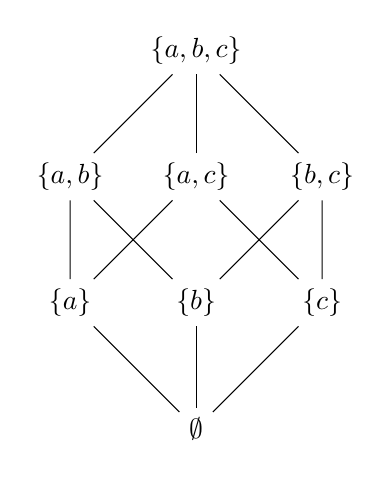
\begin{tikzpicture}[scale=0.8]
    \node (a) at (0,0) {$\emptyset$};
    \node (b) at (-2,2) {$\{a\}$};
    \node (c) at (0,2) {$\{b\}$};
    \node (d) at (2,2) {$\{c\}$};
    \node (e) at (-2,4) {$\{a,b\}$};
    \node (f) at (0,4) {$\{a,c\}$};
    \node (g) at (2,4) {$\{b,c\}$};
    \node (h) at (0,6) {$\{a,b,c\}$};

    \draw (a) -- (b);
    \draw (a) -- (c);
    \draw (a) -- (d);
    \draw (b) -- (e);
    \draw (b) -- (f);
    \draw (c) -- (e);
    \draw (c) -- (g);
    \draw (d) -- (f);
    \draw (d) -- (g);
    \draw (e) -- (h);
    \draw (f) -- (h);
    \draw (g) -- (h);
  \end{tikzpicture}
  \caption{Hasse diagram for the partially ordered set $\langle \setof{\{a, b, c\}}, \subseteq \rangle$.}
  \labfig{hasse_diagram}
  \end{marginfigure}

A finite partially ordered set $\langle D, \sqsubseteq \rangle$ can be represented by a Hasse diagram such as the one in~\reffig{hasse_diagram}: each element $x \in X$ is uniquely represented by a node of the diagram, and there is an edge from a node $x \in X$ to a node $y \in X$ if $y$ covers $x$, that is, $x \sqsubseteq y$ and there exists no $z \in X$ such that $x \sqsubseteq z \sqsubseteq y$. Hasse diagrams are usually drawn placing the elements higher than the elements they cover.

\begin{remark}
  Note that, for \emph{any} set of elements $X$, $\langle X, \subseteq \rangle$ is a poset ordered by set inclusion $\subseteq$.
\end{remark}

\begin{marginfigure}
  \centering
  \begin{tikzpicture}
    \node (a) at (-1,0) {$a$};
    \node (b) at (-2,2) {$b$};
    \node (c) at (0,2) {$c$};

    \draw (a) -- (b);
    \draw (a) -- (c);
  \end{tikzpicture}
  \caption{Hasse diagram for the poset $\langle \setof{a, b, c}, \{(a, b), (a, c)\}\rangle$.}
  \labfig{posetA}
  \end{marginfigure}

\begin{marginfigure}
  \centering
  \begin{tikzpicture}
    \node (a) at (0,0) {$a$};
    \node (b) at (0,2) {$b$};
    \node (c) at (2,0) {$c$};
    \node (d) at (2,2) {$d$};

    \draw (a) -- (b);
    \draw (c) -- (d);
  \end{tikzpicture}
  \caption{Hasse diagram for the poset $\langle \setof{a, b, c, d}, \{(a, b), (c, d)\}\rangle$.}
  \labfig{posetB}
  \end{marginfigure}

\begin{example}
  To draw a few examples: \reffig{posetA} represents the poset $\langle \setof{a, b, c}, \{(a, b), (a, c)\}\rangle$; and \reffig{posetB} represents the poset $\langle \setof{a, b, c, d}, \{(a, b), (c, d)\}\rangle$.
\end{example}

Next we introduce some important concepts related to partially ordered sets.
Let $\langle X, \sqsubseteq \rangle$ be a partially ordered set and $X'$ be a subset of $X$.
\begin{description}
  \item[Greatest Element] When it exists, the greatest element of $X$ (or top) is denoted by $\top$: $\forall x \in X.\spacer x \sqsubseteq \top$.
  \marginnote{Note that, any partially ordered set can always be equipped with a least (resp. greatest) element by adding a new element that is smaller (resp. greater) than every other element.}
  \item[Least Element] When it exists, the least element of $X$ (or bottom) is denoted by $\bot$: $\forall x \in X.\spacer \bot \sqsubseteq x$.
  \item[Maximal Element] An element $x \in X$ is maximal in $X$ if, $\forall y \in X.\spacer x \sqsubseteq y$ implies $x = y$.
  \item[Maximum] A maximal element $x \in X$ is a maximum of $X$ if it is unique.
  \item[Minimal Element] Dually, an element $x \in X$ is minimal in $X$ if, $\forall y \in X.\spacer y \sqsubseteq x$ implies $x = y$.
  \item[Minimum] A minimal element $x \in X$ is a minimum of $X$ if it is unique.
  \item[Upper Bound] An element $x \in X$ is an upper bound of $X'$ if, $\forall y \in X'.\spacer y \sqsubseteq x$.
  \item[Lower Bound] Dually, an element $x \in X$ is a lower bound of $X'$ if, $\forall y \in X'.\spacer x \sqsubseteq y$.
  \item[Least Upper Bound] When it exists, the least upper bound (lub) of $X'$ is denoted by $\join X'$: it is an upper bound $x \in X$ of $X'$ such that, for every upper bound $x' \in X$ of $X'$, $x \sqsubseteq x'$.
  \item[Greatest Lower Bound] When it exists, the greatest lower bound (glb) of $X'$ is denoted by $\meet X'$: it is a lower bound $x \in X$ of $X'$ such that, for every lower bound $x' \in X$ of $X'$, $x' \sqsubseteq x$.
\end{description}

% Let $\langle D, \leq \rangle$ be a partially ordered set. The least element of the poset, when it exists, is denoted by $\bot$: $\forall d \in D : \bot \leq d$. Similarly, the greatest element of the poset, when it exists, is denoted by $\top$: $\forall d \in D : d \leq \top$. Note that any partially ordered set can always be equipped with a least (resp. greatest) element by adding a new element that is smaller (resp. greater) than every other element. Let $X \subseteq D$. A maximal element of $X$ is an element $d \in X$ such that, for each $x \in X$, $x \leq d$. When $X$ has a unique maximal element, it is called maximum and it is denoted by $\max X$. Dually, a minimal element of $X$ is an element $d \in X$ such that, for each $x \in X$, $d \leq x$. When $X$ has a unique minimal element, it is called minimum and it is denoted by $\min X$. An upper bound of $X$ is an element $d \in D$ (not necessarily belonging to $X$) such that, for each $x \in X$, $x \leq d$. The least upper bound (or lub, or supremum) of $X$ is an upper bound $d \in D$ of $X$ and such that, for every upper bound $d' \in D$ of $X$, $d \leq d'$. When it exists, it is unique and denoted by $\bigvee X$ (or $\sup X$). Dually, a lower bound of $X$ is an element $d \in D$ such that, for each $x \in X$, $d \leq x$. The greatest lower bound (or glb, or infimum) of $X$ is a lower bound $d \in D$ of $X$ such that, for every lower bound $d' \in D$ of $X$, $d' \leq d$. When it exists, it is unique and denoted by $\bigwedge X$ (or $\inf X$). Note that the notion of maximal element, maximum, and least upper bound (resp. minimal element, minimum, and greatest lower bound) are different, as illustrated by the following example.

% \begin{example}
% Let us consider the partially ordered set $\langle \setof(\{a, b, c\}), \subseteq \rangle$ represented in \reffig{hasse_diagram} and the subset $X' \defeq \{\{a\}, \{b\}, \{c\}, \{a, b\}, \{a, c\}, \{b, c\}\}$, . The maximal elements of $X$ are $\{a, b\}$, $\{a, c\}$, and $\{b, c\}$. Thus, the maximum $\max X$ of $X$ does not exist, while its least upper bound is $\sup X = \{a, b, c\}$. Similarly, the minimal elements of $X$ are $\{a\}$, $\{b\}$, and $\{c\}$. Thus, the minimum $\min X$ of $X$ does not exist, while its greatest lower bound is $\inf X = \emptyset$.
% \end{example}


\begin{marginfigure}
  \centering
  \begin{tikzpicture}[scale=0.8]
    \node (a) at (0,0) {$\emptyset$};
    \node (b) at (-2,2) {$\{a\}$};
    \node (c) at (0,2) {$\{b\}$};
    \node (d) at (2,2) {$\{c\}$};
    \node (e) at (-2,4) {$\{a,b\}$};
    \node (f) at (0,4) {$\{a,c\}$};
    \node (g) at (2,4) {$\{b,c\}$};
    \node (h) at (0,6) {$\{a,b,c\}$};

    \draw (a) -- (b);
    \draw (a) -- (c);
    \draw (a) -- (d);
    \draw (b) -- (e);
    \draw (b) -- (f);
    \draw (c) -- (e);
    \draw (c) -- (g);
    \draw (d) -- (f);
    \draw (d) -- (g);
    \draw (e) -- (h);
    \draw (f) -- (h);
    \draw (g) -- (h);

    % subset X'
    \draw[seabornBlue, thick, dashed, rounded corners] (-2.9, .7) rectangle (2.9, 5.3);
    \node[seabornBlue] at (3.3, 4.2) {$X'$};

    % maximals of X'
    \draw[seabornGreen, thick, dashed, rounded corners] (-2.7, 3.5) rectangle (2.7, 4.5);
    \node[seabornGreen, fill=white] at (1.8, 4.9) {Maximals};

    % minimals of X'
    \draw[seabornRed, thick, dashed, rounded corners] (-2.7, 1.5) rectangle (2.7, 2.5);
    \node[seabornRed, fill=white] at (-1.8, 1.1) {Minimals};

    % lub of X'
    \draw[seabornYellow, thick, dashed, rounded corners] (-0.4, -0.5) rectangle (0.4, .5);
    \node[seabornYellow, fill=white] at (1, 0) {Lub};

    % glb of X'
    \draw[seabornOrange, thick, dashed, rounded corners] (-0.9, 5.5) rectangle (0.9, 6.5);
    \node[seabornOrange, fill=white] at (1.4, 6) {Glb};
  \end{tikzpicture}
  \caption{Maximal and minimal elements of the subset $X'$, as well as its least upper and greatest lower bounds.}
  \labfig{elements}
  \end{marginfigure}

\begin{example}
  Let us consider the partially ordered set $\langle \setof{\{a, b, c\}}, \subseteq \rangle$ and the subset $X' \defeq \{\{a\}, \{b\}, \{c\}, \{a, b\}, \{a, c\}, \{b, c\}\}$, represented in blue in \reffig{elements}.
  The maximal elements of $X'$ are $\{a, b\}$, $\{a, c\}$, and $\{b, c\}$, labelled ``Maximals'' in green. As we notice, the maximum of $X'$ does not exist, while its least upper bound is $\join X' = \{a, b, c\}$, labelled ``Lub'' in yellow.
  The minimal elements of $X'$ are $\{a\}$, $\{b\}$, and $\{c\}$, labelled ``Minimals'' in red. As we notice, the minimum of $X'$ does not exist, while its greatest lower bound is $\meet X' = \emptyset$, labelled ``Glb'' in orange.
\end{example}





\subsection{Lattices}
\labsec{lattices}

Lattices are posets that require every nonempty finite subset to have both a least upper bound and a greatest lower bound.

\marginnote{Any totally ordered set is a lattice.}
\begin{definition}[Lattice]\labdef{lattice}
  A \emph{lattice} $\langle X, \sqsubseteq, \join, meet \rangle$ is a poset where $\forall x, x'\in X$ the least upper bound $\join\{x, x'\}$ and the greatest lower bound $\meet\{x, x'\}$ exist.
\end{definition}

Complete lattices are lattices that additionally require every (possibly infinite) subset to have both a least upper bound and a greatest lower bound.

\begin{definition}[Complete Lattice]\labdef{complete-lattice}
  A \emph{complete lattice} $\langle X, \sqsubseteq, \join, \meet, \bot, \top \rangle$ is a lattice where $\forall X' \subseteq X$ the least upper bound $\join X'$ and the greatest lower bound $\meet X'$ exist.
  Complete lattices have both a least element $\bot \defeq \meet X$ and a greatest element $\top \defeq \join X$.
\end{definition}

\begin{marginfigure}
  \centering
  \begin{tikzpicture}
    \node (0) at (0,0) {$0$};
    \node (1) at (0,1) {$1$};
    \node (2) at (0,2) {$2$};
    \node (rest) at (0,3) {$\vdots$};

    \draw (0) -- (1);
    \draw (1) -- (2);
    \draw (2) -- (rest);
  \end{tikzpicture}
  \caption{Hasse diagram for the lattice $\langle \N, \le, \max, \min \rangle$.}
  \labfig{N}
  \end{marginfigure}

\begin{marginfigure}
  \centering
  \begin{tikzpicture}
    \node (0) at (0,0) {$0$};
    \node (1) at (0,1) {$1$};
    \node (2) at (0,2) {$2$};
    \node (rest) at (0,3) {$\vdots$};
    \node (inf) at (0,4) {$+\infty$};

    \draw (0) -- (1);
    \draw (1) -- (2);
    \draw (2) -- (rest);
    \draw (rest) -- (inf);
  \end{tikzpicture}
  \caption{Hasse diagram for the complete lattice $\langle \Nplus, \le, \max, \min, 0, +\infty \rangle$.}
  \labfig{Nplus}
  \end{marginfigure}


\begin{example}
  The posets of \reffig{posetA} and \reffig{posetB} are not lattices, as they do not have a least upper bound for every pair of elements, \eg, $\join\{a, b\}$ does not exist in \reffig{posetA} and $\join\{a, c\}$ does not exist in \reffig{posetB}.
%
  \reffig{hasse_diagram} represents a complete lattice with a finite number of elements.
  The poset $\langle \N, \le \rangle$ is a lattice, as every pair of natural numbers has a least upper bound and a greatest lower bound, but it is not a complete lattice, as $\join \N$ does not exist.
  Lastly, the poset $\langle \Nplus, \le \rangle$ where $+\infty$ is greater than any natural number is indeed a complete lattice.
  \reffig{N} shows the Hasse diagram for $\langle \Nplus, \le \rangle$ and \reffig{Nplus} the one for $\langle \Nplus, \le \rangle$.
\end{example}

\begin{remark}
  Given any set of elements $X$, the power set $\langle \setof{X}, \subseteq, \setjoin, \setmeet, \emptyset, X \rangle$ is a complete lattice.
\end{remark}


\subsection{Functions}
\labsec{functions}

% A partial function $f$ from a set $A$ to a set $B$, written $f : A \rightharpoonup B$, is a binary relation between $A$ and $B$ that pairs each element $x \in A$ with no more than one element $y \in B$. The set of all partial functions from a set $A$ to a set $B$ is denoted by $A \rightharpoonup B$. We write $f(x) = y$ if there exists an element $y$ such that $(x, y) \in f$, and we say that $f(x)$ is defined, otherwise we say that $f(x)$ is undefined. Given a partial function $f : A \rightharpoonup B$, we define its domain as $\text{dom}(f) \triangleq \{x \in A \mid \exists y \in B : f(x) = y\}$. The totally undefined function, denoted by $\emptyset$, has the empty set as domain: $\text{dom}(\emptyset) = \emptyset$. The join of two partial functions $f_1 : A \rightharpoonup B$ and $f_2 : A \rightharpoonup B$ with disjoint domains, denoted by $f_1 \cup f_2 : A \rightharpoonup B$, is defined as follows:
% \[
% (f_1 \cup f_2)(x) \triangleq
% \begin{cases}
% f_1(x) & x \in \text{dom}(f_1) \\
% f_2(x) & x \in \text{dom}(f_2) \\
% \text{undefined} & \text{otherwise}
% \end{cases}
% \]
% where $\text{dom}(f_1) \cap \text{dom}(f_2) = \emptyset$.

% A (total) function $f$ from a set $A$ to a set $B$, written $f : A \to B$, is a partial function that pairs each $x \in A$ with exactly one element $y \in B$. Equivalently, a (total) function $f : A \to B$ is a partial function such that $\text{dom}(f) = A$. The set of all functions from a set $A$ to a set $B$ is denoted by $A \to B$.

% We sometimes denote functions using the lambda notation $\lambda x \in A. f(x)$, or more concisely $\lambda x. f(x)$.

% The composition of two functions $f : A \to B$ and $g : B \to C$ is another function $g \circ f : A \to C$ such that $\forall x \in A : (g \circ f)(x) = g(f(x))$.

% The following properties may hold for a function $f : A \to B$:
% \begin{itemize}
%     \item Injectivity: $\forall x, y \in A : f(x) = f(y) \implies x = y$
%     \item Surjectivity: $\forall y \in B : \exists x \in A : f(x) = y$
% \end{itemize}

% A bijective function, also called isomorphism, is both injective and surjective. Two sets $A$ and $B$ are isomorphic if there exists a bijective function $f : A \to B$. The inverse of a bijective function $f : A \to B$ is the bijective function $f^{-1} : B \to A$ defined as $f^{-1} \triangleq \{(b, a) \mid (a, b) \in f\}$.

% Let $\langle D_1, \leq_1 \rangle$ and $\langle D_2, \leq_2 \rangle$ be partially ordered sets. A function $f : D_1 \to D_2$ is said to be monotonic when, for each $x, y \in D_1, x \leq_1 y \implies f(x) \leq_2 f(y)$. It is continuous (or Scott-continuous) when it preserves existing least upper bounds of chains, that is, for each chain $C \subseteq D_1$, if $\bigvee C$ exists then $f(\bigvee C) = \bigvee \{f(x) \mid x \in C\}$. Dually, it is co-continuous when it preserves existing greatest lower bounds of chains, that is, if $\bigwedge C$ exists then $f(\bigwedge C) = \bigwedge \{f(x) \mid x \in C\}$. A complete $\bigvee$-morphism (resp. complete $\bigwedge$-morphism) preserves existing least upper bounds (resp. greatest lower bounds) of arbitrary non-empty sets.

% Given a complete lattice $\langle D, \leq, \bigvee, \bigwedge, \bot, \top \rangle$ (resp. a lattice, a cpo, a poset) and a set $S$, the set $S \to D$ of all functions from $S$ to $D$ inherits the complete lattice (resp. lattice, cpo, poset) structure of $D$: $\langle S \to D, \leq, \bigvee, \bigwedge, \bot, \top \rangle$ where the dotted operators are defined by pointwise lifting:
% \[
% \begin{aligned}
% f \leq g & \triangleq \forall s \in S : f(s) \leq g(s) \\
% \bigvee X & \triangleq \lambda s. \bigvee \{f(s) \mid f \in X\} \\
% \bigwedge X & \triangleq \lambda s. \bigwedge \{f(s) \mid f \in X\} \\
% \bot & \triangleq \lambda s. \bot \\
% \top & \triangleq \lambda s. \top
% \end{aligned}
% \]

\subsection{Fixpoints}
\labsec{fixpoints}

% Given a partially ordered set $\langle D, \leq \rangle$ and a function $f : D \to D$, a fixpoint of $f$ is an element $x \in D$ such that $f(x) = x$. An element $x \in D$ such that $x \leq f(x)$ is called a pre-fixpoint while, dually, a post-fixpoint is an element $x \in D$ such that $f(x) \leq x$. The least fixpoint of $f$, written $\text{lfp} \, f$, is a fixpoint of $f$ such that, for every fixpoint $x \in D$ of $f$, $\text{lfp} \, f \leq x$. We write $\text{lfp}_d f$ for the least fixpoint of $f$ which is greater than or equal to an element $d \in D$. Dually, we define the greatest fixpoint of $f$, denoted by $\text{gfp} \, f$, and the greatest fixpoint of $f$ smaller than or equal to $d \in D$, denoted by $\text{gfp}_d f$. When the order $\leq$ is not clear from the context, we explicitly write $\text{lfp}_{\leq} f$ and $\text{gfp}_{\leq} f$.

% We now recall a fundamental theorem due to Alfred Tarski:

% \begin{theorem}[Tarski's Fixpoint Theorem]
% The set of fixpoints of a monotonic function $f : D \to D$ over a complete lattice is also a complete lattice.
% \end{theorem}
% \begin{proof}
% See \cite{Tarski1955}.
% \end{proof}

% In particular, the theorem guarantees that $f$ has a least fixpoint $\text{lfp} \, f = \bigwedge \{x \in D \mid f(x) \leq x\}$ and a greatest fixpoint $\text{gfp} \, f = \bigvee \{x \in D \mid x \leq f(x)\}$.

% However, such fixpoint characterizations are not constructive. An alternative constructive characterization is often attributed to Stephen Cole Kleene:

% \begin{theorem}[Kleene's Fixpoint Theorem]
% Let $\langle D, \leq \rangle$ be a complete partial order and let $f : D \to D$ be a Scott-continuous function. Then, $f$ has a least fixpoint which is the least upper bound of the increasing chain
% \[
% \bot \leq f(\bot) \leq f(f(\bot)) \leq f(f(f(\bot))) \leq \cdots
% \]
% \ie, $\text{lfp} \, f = \bigvee \{f^n(\bot) \mid n \in \mathbb{N}\}$.
% \end{theorem}

% In case of monotonic but not continuous functions, a theorem by Patrick Cousot and Radhia Cousot expresses fixpoints as limits of possibly transfinite iteration sequences:

% \begin{theorem}
% Let $f : D \to D$ be a monotonic function over a complete partial order and let $d \in D$ be a pre-fixpoint. Then, the iteration sequence:
% \[
% f^\alpha \triangleq
% \begin{cases}
% d & \alpha = 0 \\
% f(f^\beta) & \alpha = \beta + 1 \\
% \bigvee \{f^\beta \mid \beta < \alpha\} & \text{otherwise}
% \end{cases}
% \]
% converges towards the least fixpoint $\text{lfp}_d f$.
% \end{theorem}
% \begin{proof}
% See \cite{Cousot1979}.
% \end{proof}

% In the following, the partial order between the fixpoint iterates is called computational order, in order to distinguish it from the approximation order defined in the next Section 2.2.2.


\begin{definition}[Upper Closure Operator]\labdef{upper-closure-operator}
  An \emph{upper closure operator} on a poset $\defposet$ is an operator $\rho\in\defposet\to\defposet$ which is monotone, idempotent, and extensive ($\foralldef{\defposetelem \in \defposet}{\defposetelem \le P \rho(\defposetelem)}$).
\end{definition}

\section{Notations of Abstract Interpretation}
\labsec{notations-of-abstract-interpretation}

\subsection{Transition System}
\labsec{transition-system}

\begin{definition}[State]\labdef{state}
  \begin{align*}
    \state \IN \variables \to \values
  \end{align*}
\end{definition}

\subsection{Maximal Trace Semantics}
\labsec{maximal-trace-semantics}

\begin{definition}[Maximal Trace Semantics]\labdef{maximal-trace-semantics}
  \begin{align*}
    \tracesemanticsnoparam &\DefeQ \lfp \tracetransformer \\
    \tracetransformer(\defsetoftraces) &\DefeQ \finalstates \setjoin (\mergesequences{\transitionrelation}{\defsetoftraces})
  \end{align*}
\end{definition}

\subsection{Collecting Semantics}
\labsec{collecting-semantics}

\begin{definition}[Collecting Semantics]\labdef{collecting-semantics}
  \begin{align*}
    \collectingsemanticsnoparam &\DefeQ \{\spacearound{\tracesemanticsnoparam}\}
  \end{align*}

\end{definition}

\subsection{Verification Framework}
\labsec{verification-framework}

\begin{definition}[Validation]\labdef{validation}
  \begin{align*}
    \defprogram \satisfies \defproperty \IfF \collectingsemantics \subseteq \defproperty
  \end{align*}
\end{definition}

\subsection{Fixpoint Induction}
\labsec{fixpoint-induction}

\subsection{Hierarchy of Semantics}
\labsec{hierarchy-of-semantics}

\subsection{Galois Connection}
\labsec{galois-connection}

\subsection{Reachable State Semantics}
\labsec{reachable-state-semantics}

\subsection{Fixpoint Transfer}
\labsec{fixpoint-transfer}

\subsection{Fixpoint Approximation}
\labsec{fixpoint-approximation}

\subsection{Widening}
\labsec{widening}

\subsection{Narrowing}
\labsec{narrowing}


\section{A Small Imperative Language}
\labsec{a-small-imperative-language}

\subsection{Syntax}
\labsec{syntax}

\subsection{Maximal Trace Semantics}
\labsec{maximal-trace-semantics}

\subsection{Numerical Abstract Domains}
\labsec{numerical-abstract-domains}

\subsubsection*{Sign}

\subsubsection*{Boxes}

\subsubsection*{Conjunctions of Linear Constraints}

\subsection{Reduced Product}
\labsec{reduced-product}

\subsection{Forward Reachability State Semantics}
\labsec{forward-reachability-state-semantics}

\subsection{Backward Reachability State Semantics}
\labsec{backward-reachability-state-semantics}

\begin{definition}[Validation]
  \labdef{validation}
  \begin{align}
    \labeq{validation}
    \defprogram \satisfies \defproperty \iff \collectingsemantics \subseteq \defproperty
  \end{align}
\end{definition}

\begin{definition}[Collecting Semantics]
  \labdef{collecting-semantics}
  \begin{align}
    \labeq{collecting-semantics}
    \collectingsemanticsnoparam \defeq \{ \dependencysemanticsnoparam \}
  \end{align}
\end{definition}

\begin{definition}[Dependency Semantics]
  \labdef{dependency-semantics}
  \begin{align*}
    \dependencysemanticsnoparam \DefeQ \setdef{\inputoutputtuple{\defseq}}{\defseq\in\tracesemanticsnoparam}
  \end{align*}
\end{definition}

\begin{definition}[Backward Semantics]\labdef{backward-semantics}
\begin{align*}
&\backwardsemanticsnoparam \semanticsof{\skipstmt}\defabstractvalue \DefeQ
\defabstractvalue
\\
&\backwardsemanticsnoparam \semanticsof{\assignstmt}\defabstractvalue \DefeQ
\abstractdomainsubstitute{\defvariable}{\defaexp}\defabstractvalue
\\
&\backwardsemanticsnoparam \semanticsof{\assertstmt}\defabstractvalue \DefeQ
\abstractdomainfilter\semanticsof{\defbexp}\defabstractvalue
\\
&\backwardsemanticsnoparam \semanticsof{\ifstmt[\defstmt][\defstmt']}\defabstractvalue \DefeQ
\\
&\quad \abstractdomainfilter\semanticsof{\defbexp}(\backwardsemanticsnoparam \semanticsof{\defstmt}\defabstractvalue) \spacearound{\abstractdomainjoin} \abstractdomainfilter\semanticsof{\neg\defbexp}(\backwardsemanticsnoparam \semanticsof{\defstmt'}\defabstractvalue)
\\
&\backwardsemanticsnoparam \semanticsof{\whilestmt}\defabstractvalue \DefeQ \lim_n \abstractdomainfixpoint_n \\
&\quad \abstractdomainfixpoint_0 \DefeQ \defabstractvalue \\
&\quad \abstractdomainfixpoint_{n+1} \DefeQ \abstractdomainfixpoint_n \spacearound{\abstractdomainwidening} \abstractdomainfixpoint(\abstractdomainfixpoint_n) \\
&\quad \abstractdomainfixpoint(\defotherabstractvalue) \DefeQ \abstractdomainfilter\semanticsof{\neg\defbexp}\defabstractvalue \spacearound{\abstractdomainjoin} \abstractdomainfilter\semanticsof{\defbexp}(\backwardsemanticsnoparam \semanticsof{\defstmt}\defotherabstractvalue)
\\
&\backwardsemanticsnoparam \semanticsof{\compstmt[\defstmt][\defstmt']}\defabstractvalue \DefeQ
\backwardsemanticsnoparam \semanticsof{\defstmt}( \backwardsemanticsnoparam \semanticsof{\defstmt'}\defabstractvalue)
\end{align*}
\end{definition}

\begin{marginlisting}
  \caption{Landing alarm system}
  \labprog{landing-alarm-system}
  \vspace{\lineheight}
\begin{lstlisting}[
  language=customPython,
  style=mystyle,]
landing_coeff =
  abs(angle) + speed
if landing_coeff < 2:
  risk = 0
else if landing_coeff > 5:
  risk = 3
else:
  risk =
    floor(landing_coeff) - 2
  \end{lstlisting}
\end{marginlisting}
